
\chapter{Results} 

\label{Chapter5}

%----------------------------------------------------------------------------------------

In this chapter we discuss the results obtained with our model. First, we analyze how the model works in a given (original) resolution, so that we can be confident about its performance. Then, we consider how the accuracy changes with the resolution and within the categories. Finally, we discuss the cost en environment impact around Satellite imagery to analyze the world. 

\section{Transfer Learning on Aerial Imagery}

\section{Man-made Structures Detection at Different Scale}

\begin{sidewaystable}
    \centering
	\begin{tabular}{rrrrrrrrrrr}
\toprule
res. & \multicolumn{2}{c}{All categories} & \multicolumn{2}{c}{agriculture} & \multicolumn{2}{c}{forest-woodland} & \multicolumn{2}{c}{semi-desert} & \multicolumn{2}{c}{shrubland-grassland} \\
           &     mean acc. &    std &                 mean acc. &    std &                     mean acc. &    std &                 mean acc. &    std &                         mean acc. &    std \\
\midrule
       0.3 &   0.9585 & 0.0190 &               0.9858 & 0.0158 &                   0.8978 & 0.0269 &               0.9428 & 0.0412 &                       0.9892 & 0.0125 \\
       0.6 &   0.9383 & 0.0190 &               0.9699 & 0.0216 &                   0.8779 & 0.0269 &               0.9231 & 0.0410 &                       0.9748 & 0.0198 \\
       0.9 &   0.9347 & 0.0096 &               0.9439 & 0.0244 &                   0.8944 & 0.0561 &               0.9327 & 0.0216 &                       0.9578 & 0.0212 \\
       1.2 &   0.9271 & 0.0120 &               0.9488 & 0.0374 &                   0.9061 & 0.0373 &               0.9150 & 0.0328 &                       0.9399 & 0.0231 \\
       1.5 &   0.9288 & 0.0139 &               0.9622 & 0.0285 &                   0.8679 & 0.0383 &               0.9144 & 0.0309 &                       0.9604 & 0.0215 \\
       1.8 &   0.9224 & 0.0154 &               0.9678 & 0.0311 &                   0.8864 & 0.0650 &               0.9014 & 0.0363 &                       0.9371 & 0.0221 \\
       2.1 &   0.9108 & 0.0241 &               0.9618 & 0.0168 &                   0.8749 & 0.0454 &               0.8885 & 0.0571 &                       0.9216 & 0.0371 \\
       2.4 &   0.9120 & 0.0206 &               0.9573 & 0.0280 &                   0.8686 & 0.0590 &               0.8867 & 0.0358 &                       0.9352 & 0.0263 \\
       2.7 &   0.8952 & 0.0223 &               0.9620 & 0.0216 &                   0.8631 & 0.0191 &               0.8510 & 0.0350 &                       0.9117 & 0.0496 \\
       3.0 &   0.8893 & 0.0189 &               0.9571 & 0.0067 &                   0.8717 & 0.0197 &               0.8340 & 0.0472 &                       0.9055 & 0.0455 \\
       3.3 &   0.8957 & 0.0209 &               0.9539 & 0.0311 &                   0.8723 & 0.0479 &               0.8529 & 0.0341 &                       0.9121 & 0.0425 \\
       3.6 &   0.8784 & 0.0184 &               0.9415 & 0.0394 &                   0.8727 & 0.0442 &               0.8199 & 0.0348 &                       0.8935 & 0.0299 \\
       3.9 &   0.8819 & 0.0153 &               0.9456 & 0.0186 &                   0.8738 & 0.0330 &               0.8397 & 0.0364 &                       0.8796 & 0.0178 \\
       4.2 &   0.8804 & 0.0070 &               0.9389 & 0.0305 &                   0.8525 & 0.0267 &               0.8444 & 0.0533 &                       0.8961 & 0.0222 \\
       4.5 &   0.8715 & 0.0179 &               0.9383 & 0.0390 &                   0.8445 & 0.0308 &               0.8301 & 0.0340 &                       0.8821 & 0.0206 \\
       4.8 &   0.8690 & 0.0160 &               0.9508 & 0.0157 &                   0.8569 & 0.0517 &               0.7798 & 0.0456 &                       0.9035 & 0.0310 \\
\bottomrule
\end{tabular}

	\captionsetup{width=0.7\linewidth}
	\caption{\textbf{$0.3m$ dataset}}
\end{sidewaystable}

\begin{sidewaystable}
    \centering
	    
\begin{tabular}{rrrrrrrrrrr}
\toprule
res. & \multicolumn{2}{c}{All categories} & \multicolumn{2}{c}{agriculture} & \multicolumn{2}{c}{forest-woodland} & \multicolumn{2}{c}{semi-desert} & \multicolumn{2}{c}{shrubland-grassland} \\
           &     mean acc. &    std &                 mean acc. &    std &                     mean acc. &    std &                 mean acc. &    std &                         mean acc. &    std \\
\midrule
         2 &   0.9001 & 0.0138 &               0.9803 & 0.0306 &                   0.8991 & 0.0634 &               0.8843 & 0.0413 &                       0.8881 & 0.0430 \\
         3 &   0.9041 & 0.0246 &               0.9846 & 0.0246 &                   0.9245 & 0.0280 &               0.8742 & 0.0537 &                       0.8805 & 0.0315 \\
         4 &   0.8970 & 0.0227 &               0.9846 & 0.0246 &                   0.8743 & 0.0280 &               0.8786 & 0.0481 &                       0.9129 & 0.0222 \\
         5 &   0.8865 & 0.0391 &               0.9809 & 0.0328 &                   0.8692 & 0.0577 &               0.8821 & 0.0328 &                       0.8797 & 0.0472 \\
         6 &   0.8800 & 0.0282 &               0.9673 & 0.0352 &                   0.8685 & 0.0467 &               0.8419 & 0.0469 &                       0.9093 & 0.0508 \\
         7 &   0.8587 & 0.0350 &               0.9584 & 0.0482 &                   0.8360 & 0.0653 &               0.8468 & 0.0583 &                       0.8682 & 0.0598 \\
         8 &   0.8699 & 0.0230 &               0.9831 & 0.0289 &                   0.8788 & 0.0442 &               0.8432 & 0.0303 &                       0.8498 & 0.0335 \\
         9 &   0.8338 & 0.0148 &               0.9341 & 0.0562 &                   0.8330 & 0.0565 &               0.8086 & 0.0431 &                       0.8245 & 0.0543 \\
        10 &   0.8234 & 0.0263 &               0.9911 & 0.0253 &                   0.8159 & 0.0553 &               0.7815 & 0.0420 &                       0.8199 & 0.0700 \\
        11 &   0.8219 & 0.0249 &               0.9703 & 0.0645 &                   0.8052 & 0.0507 &               0.7901 & 0.0538 &                       0.8193 & 0.0702 \\
        12 &   0.8112 & 0.0257 &               0.9490 & 0.0333 &                   0.8178 & 0.0362 &               0.7606 & 0.0363 &                       0.8118 & 0.0814 \\
        13 &   0.8147 & 0.0369 &               0.9666 & 0.0488 &                   0.7988 & 0.0921 &               0.7719 & 0.0723 &                       0.8244 & 0.0572 \\
        14 &   0.7837 & 0.0167 &               0.9351 & 0.0690 &                   0.7682 & 0.0403 &               0.7398 & 0.0543 &                       0.7999 & 0.0397 \\
        15 &   0.7808 & 0.0245 &               0.9457 & 0.0289 &                   0.7663 & 0.0673 &               0.7257 & 0.0472 &                       0.8017 & 0.0439 \\
        16 &   0.7990 & 0.0361 &               0.9403 & 0.0635 &                   0.7680 & 0.0700 &               0.7713 & 0.0857 &                       0.8141 & 0.0764 \\
\bottomrule
\end{tabular}

	\captionsetup{width=0.7\linewidth}
	\caption{\textbf{$1m$ dataset}}
\end{sidewaystable}


\begin{figure}[h!]
	\centering
	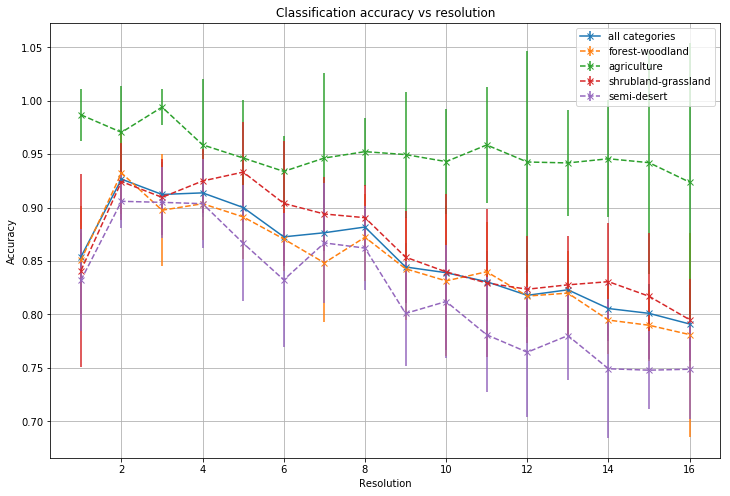
\includegraphics[width=\textwidth]{Figures/results/results_1m_all_categories.png}
	\captionsetup{width=1\linewidth}
	\caption{\textbf{$1m$ dataset}}
	\label{fig:acc_1m_all_cat}
\end{figure}

\begin{figure}[h!]
	\centering
	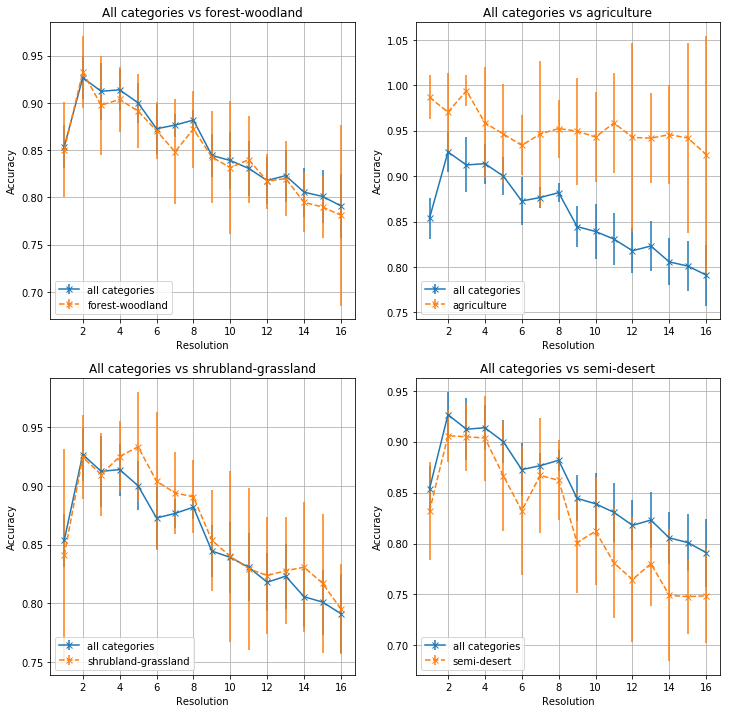
\includegraphics[width=\textwidth]{Figures/results/results_1m_by_category.png}
	\captionsetup{width=1\linewidth}
	\caption{\textbf{$1m$ dataset}}
	\label{fig:acc_1m_byl_cat}
\end{figure}



\section{Cost and Environment impact}
